\documentclass[12pt]{article}
\usepackage{graphicx}
\usepackage{amsmath}
\usepackage{amssymb}
\usepackage{color}
\usepackage{caption}
\usepackage{subcaption}
\usepackage{mdframed}
\usepackage[margin=2.5cm]{geometry}
\usepackage[superscript,biblabel]{cite}
\usepackage{url}
\numberwithin{equation}{section}
\numberwithin{figure}{section}



\begin{document}

\title{Calculating the Differential Cross Section Using IceCube Simulation Data}
\author{Ryan Hill \\
Queen Mary, University Of London Undergraduate\\
\texttt{r.l.hill@se12.qmul.ac.uk}}
\date{\today}
\maketitle
\thispagestyle{empty}
%
\graphicspath{{images/}}
%
%
\begin{abstract}
This review will summarise the work I have been doing with Dr Teppei Katori over the summer of 2015 with regards to calculating the Differential Cross Section (DCS) using simulated data from the IceCube experiment at the South Pole. We will start by reviewing the equations used to calculate each part needed for the DCS, then look at the methods implemented in the macros themselves, before finally considering what the next steps would be for the development of the code.
\end{abstract}
%
\clearpage
%
\tableofcontents
\thispagestyle{empty}
%
\clearpage
%
\setcounter{page}{1}
\section{Introduction}
\subsection{Terminology} % (fold)
\label{sub:terminology}
There are a few terms that I will be using throughout this summary which you may or may not be familiar with depending on your exposure to using ROOT or neutrino physics so I will just explain them quickly here for those who need them.\\
\begin{itemize}
    \item Macro - A Macro is a snippet of code that ROOT can run. The benefit of them is that running long pieces of code in the command line can be tedious and annoying, so macros allows for repeated use of and ease of editing commands. I will use the term macro interchangeably with program and code.
    \item Zenith angle - This is technically the angle measured from directly overhead down to the horizon with a range of [0,$\pi$] denoted by $\theta$. However, 99\% of the time if this summary mentions the zenith angle it is talking about the cosine of the zenith angle with a range of [-1,1], as this is much more useful for physical purposes.
    \item Azimuth angle- This is the rotational angle on the plane of the horizon with a range of [0,2$\pi$], commonly denoted as $\phi$.
    \item Bin - Bins are how values are represented in histograms; each bin has a height that is the count of how many data points had a value that fell between the two edge values of the bin.
\end{itemize}
% subsection terminology (end)
\subsection{Differential Cross Section}
The DCS is a very important quantity in the world of particle physics and is more useful than just the regular cross section as it quantifies the intrinsic rate of an event that can be detected at a given angle, something the scalar cross section cannot tell you. With this in mind we can see why it might be important to want to calculate this quantity. The main equation we will be using in this summary is similar to the usual DCS equation with some additional quantities due to way in which the data is simulated. That equation can be written as
\begin{equation}
	\frac{d\sigma}{dE_{\mu_i}} = \frac{\sum\limits_j U_{ij}(d_j-b_j)}{\Delta E_{\mu_i} N t\Phi\epsilon_i Sr}
	\label{eq:DCS}
\end{equation}
where $U_{ij}$ is the unfolding matrix, $d_j,b_j$ are the data and background respectively, $\Delta E$ is the energy bin width, $N$ is the number of target nuclei, $t$ is the simulated time length, $\Phi$ is the integrated neutrino flux, $\epsilon_i$ is the bin efficiency and $Sr$ is the solid angle for that bin. The outputs of the main macro, included two of the DCS for simulated IceCube data are shown in figure \ref{fig:outputs}.
\begin{figure}
	\centering
	\begin{subfigure}{0.8\textwidth}
                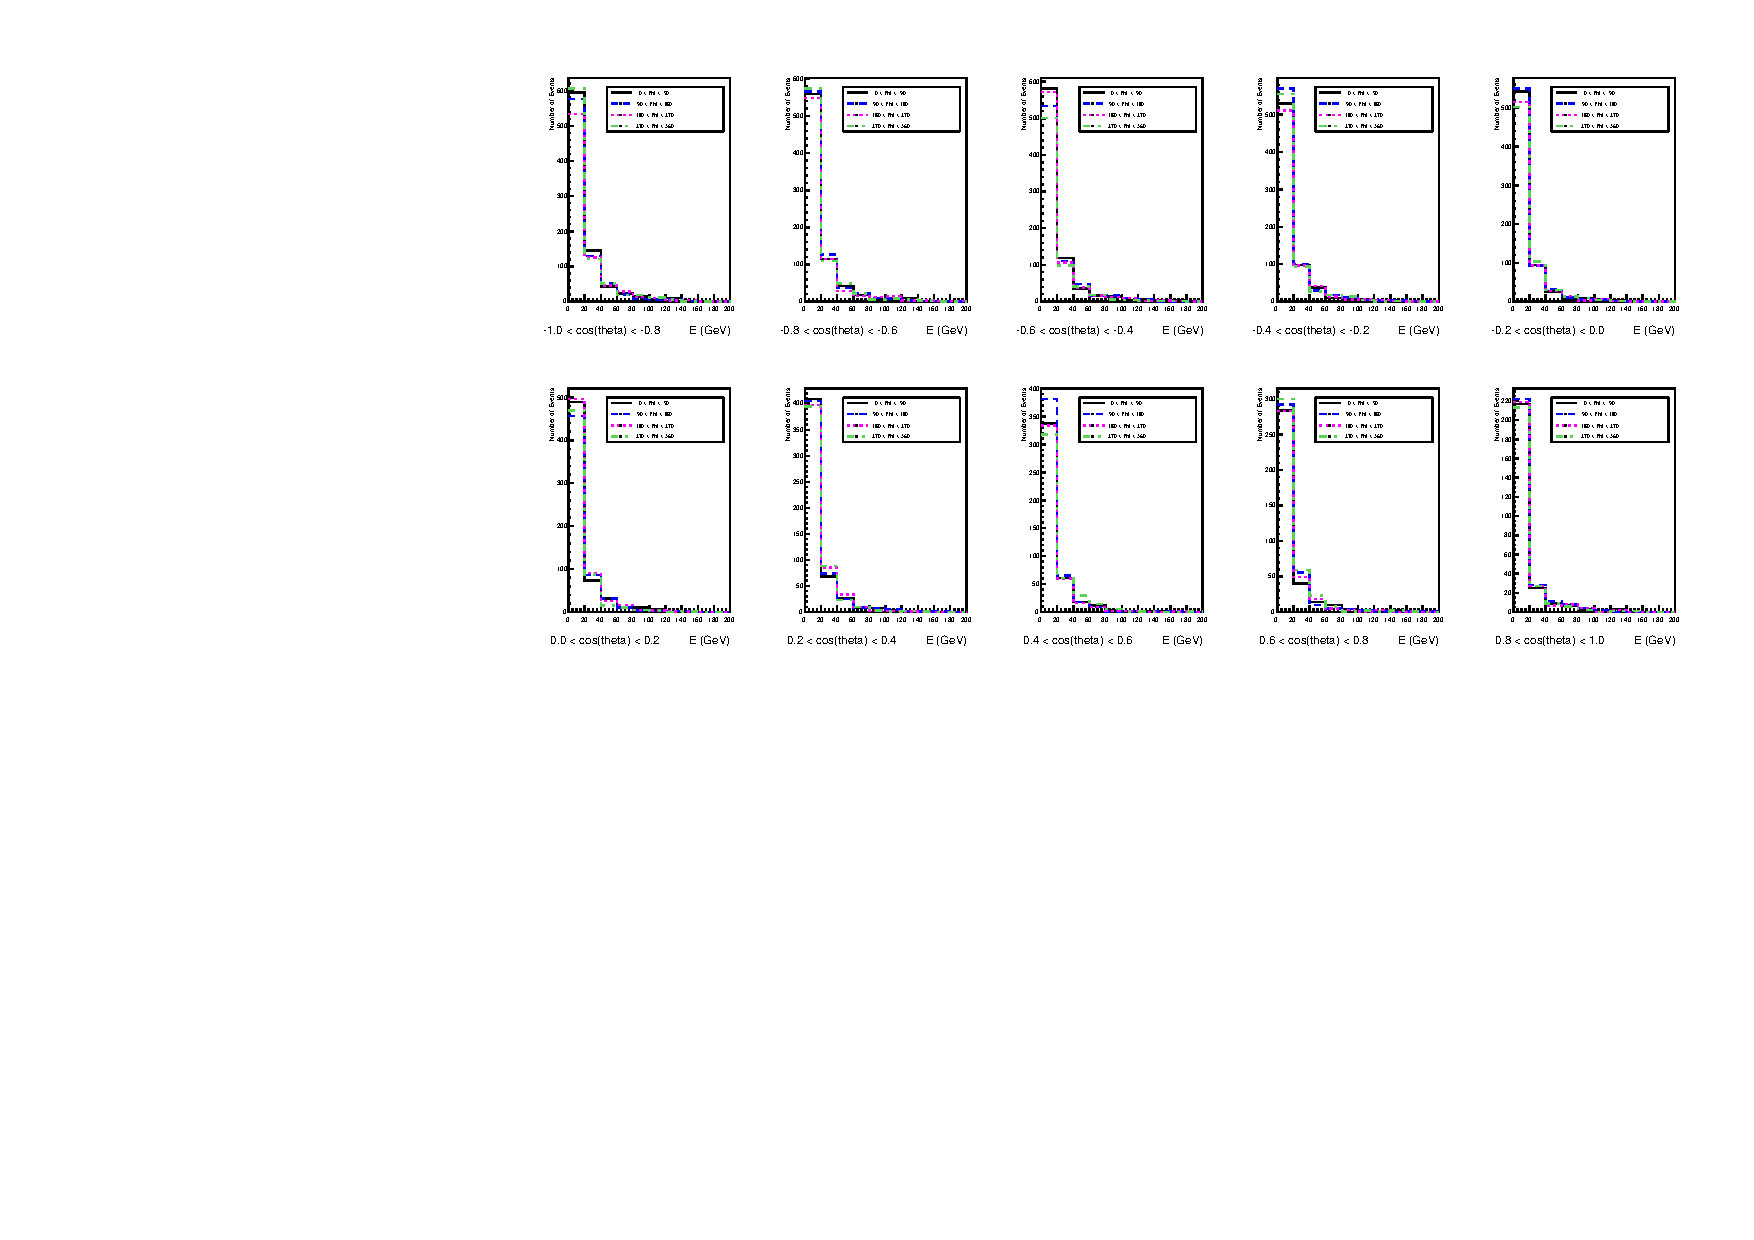
\includegraphics[scale=0.59]{MCOriginal}
                \caption{True data distribution just for comparison and sanity checks}
                \label{fig:output_orig}
    \end{subfigure}\\
    \begin{subfigure}{0.8\textwidth}
                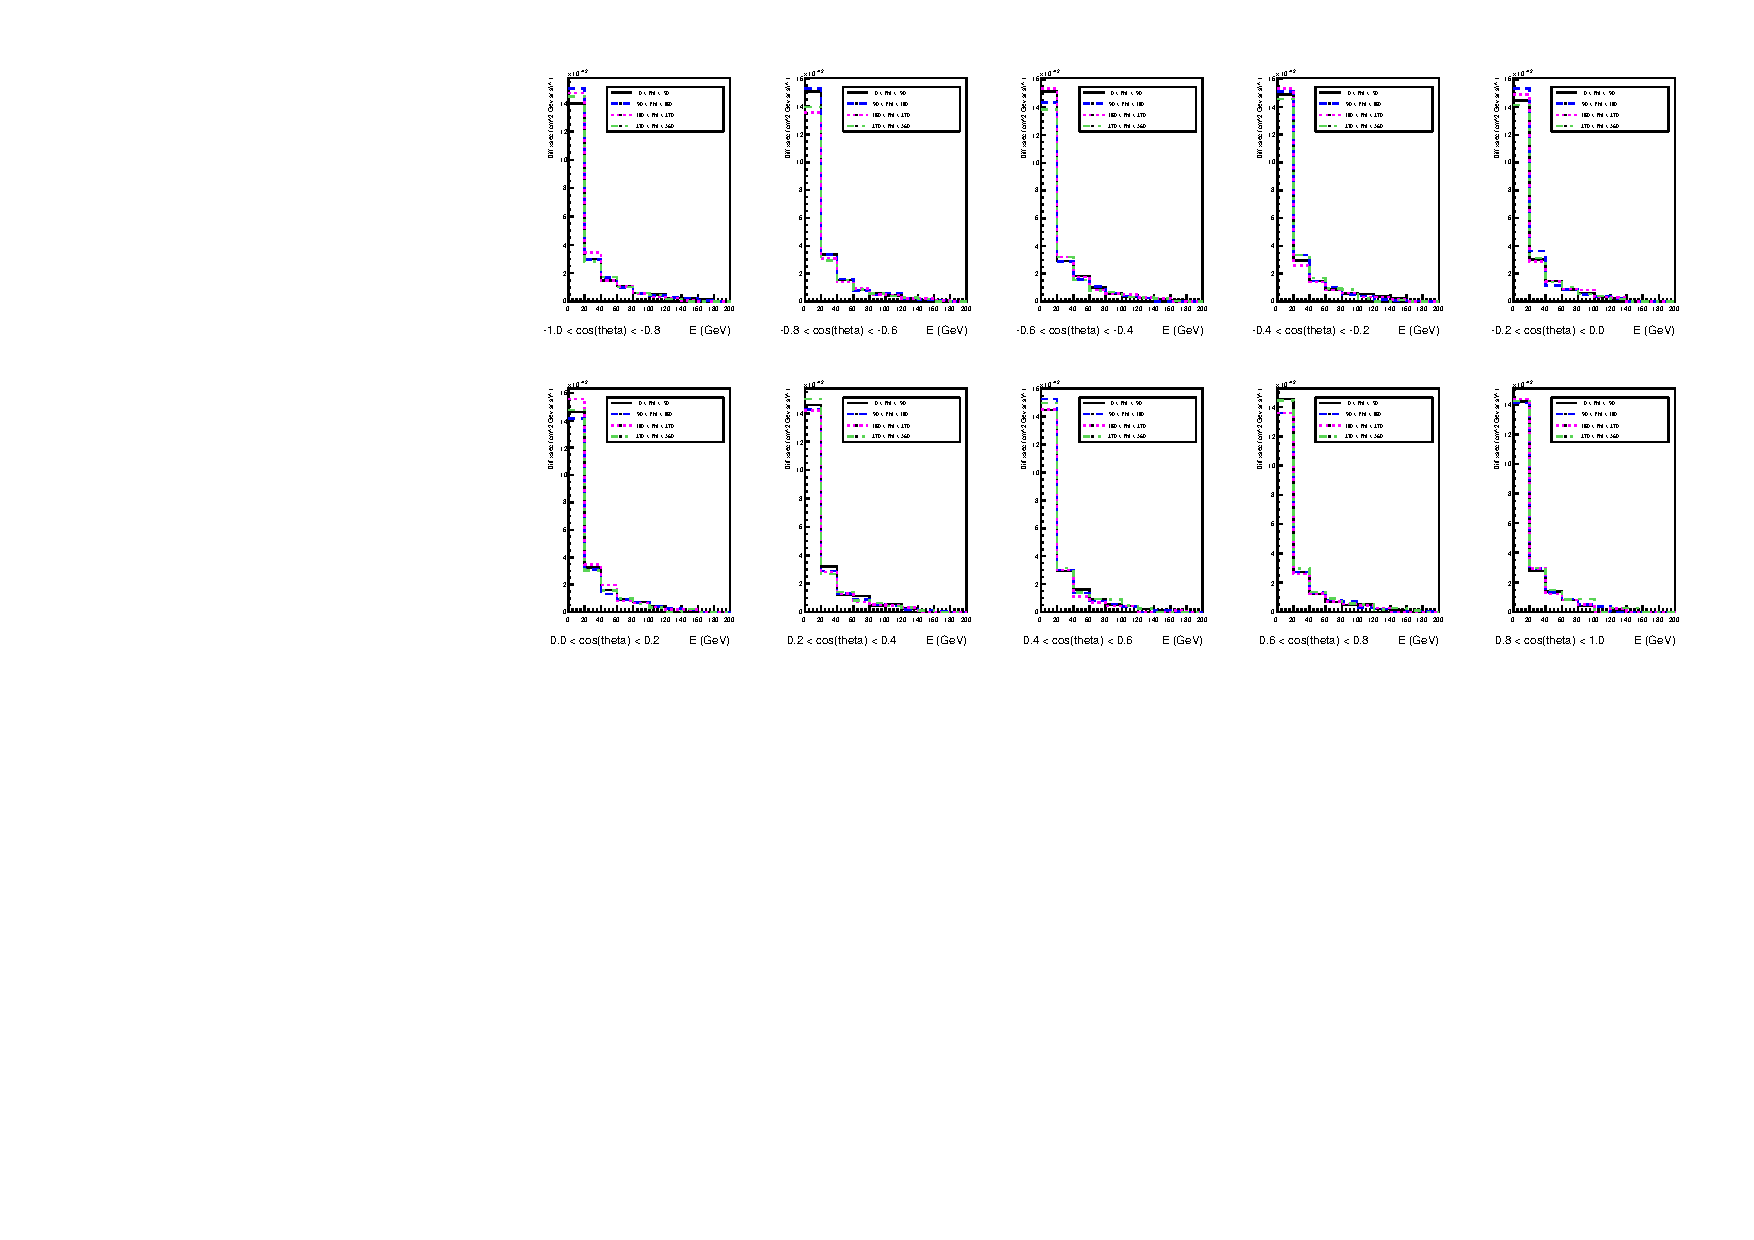
\includegraphics[scale=0.59]{MCUnfNoSmearing}
                \caption{The DCS of the fake data from the IceCube file without any smearing to the data}
                \label{fig:output_nosmear}
    \end{subfigure}\\
    \begin{subfigure}{0.8\textwidth}
                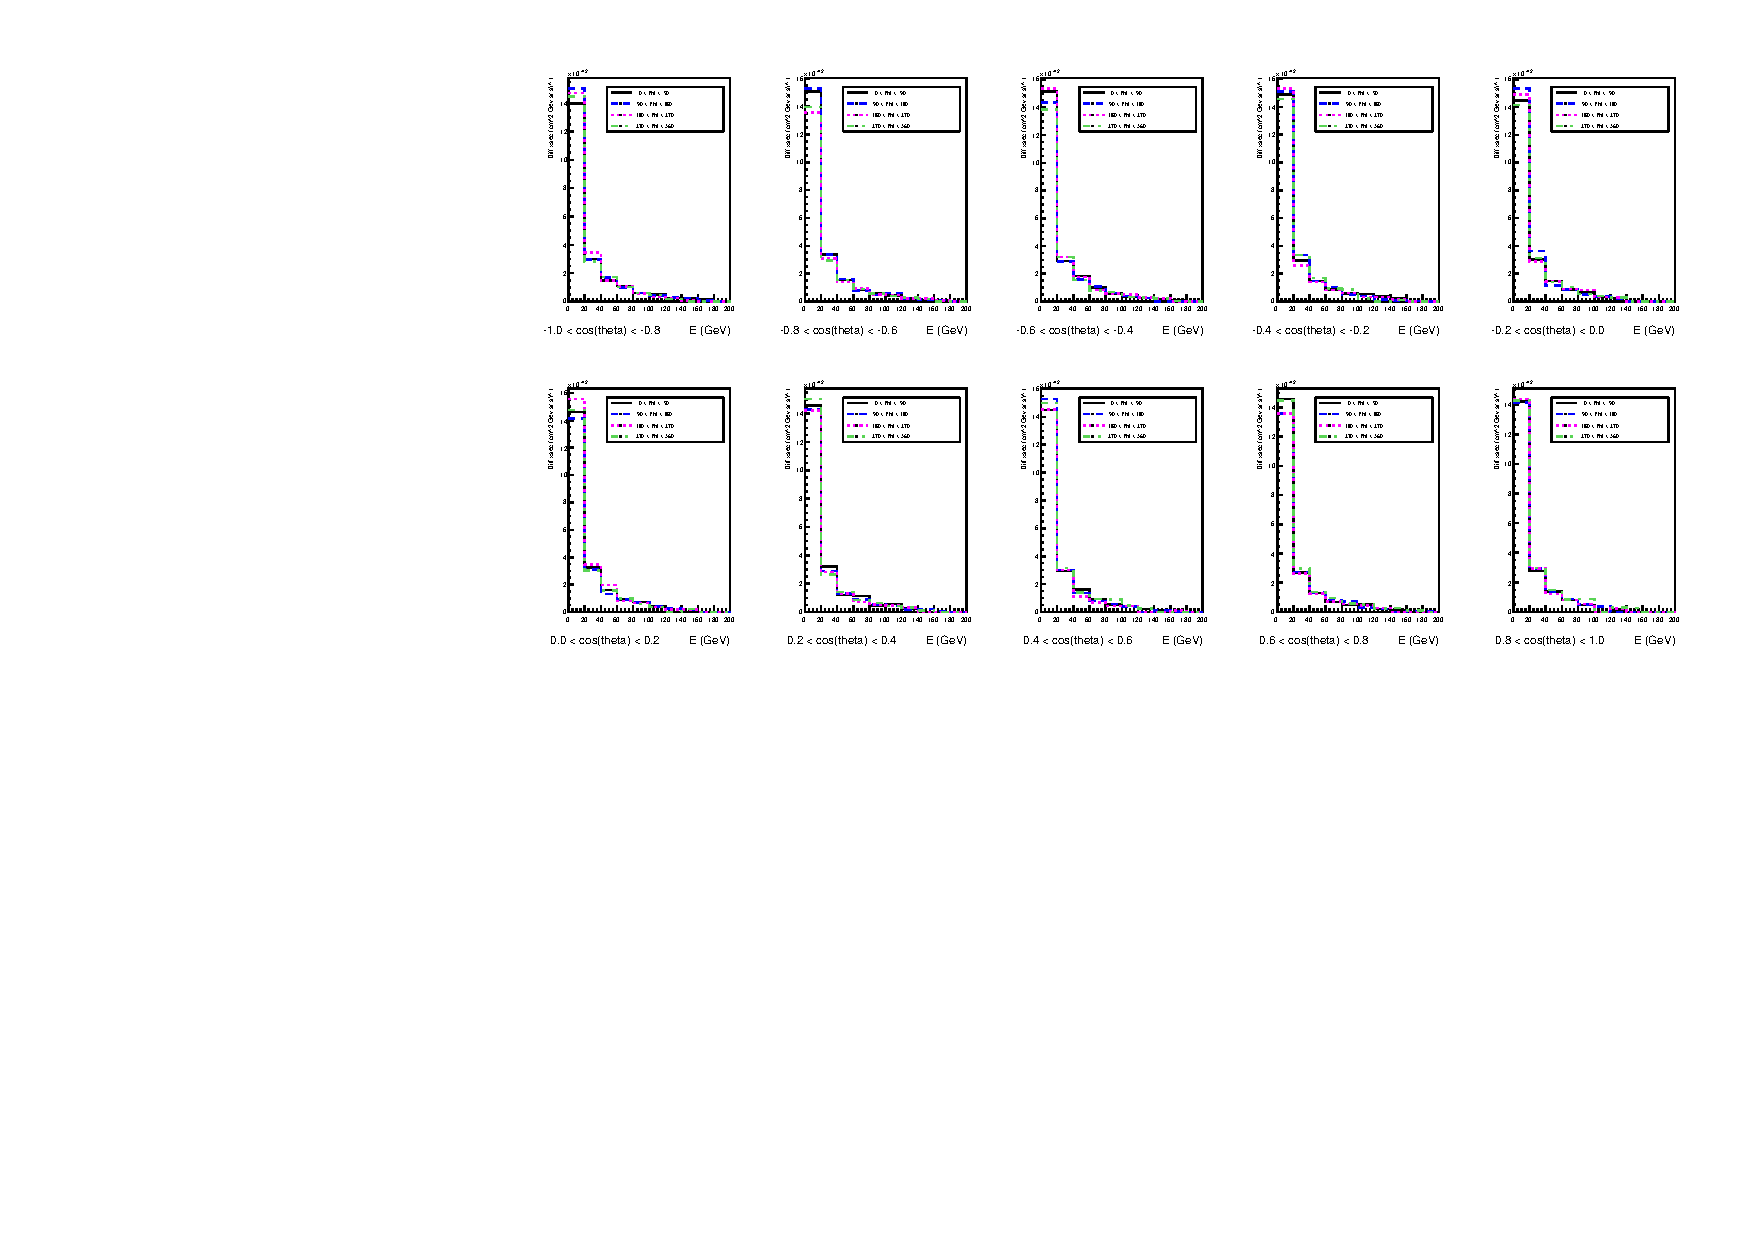
\includegraphics[scale=0.59]{MCUnfSmearing}
                \caption{The DCS of the fake data from the IceCube file with a Gaussian smear to the data}
                \label{fig:output_smear}
    \end{subfigure}
	\caption{Example outputs from the main macro in the project. Each image is split into 10 plots representing 10 cos($\theta$) ranges and each plot has 4 historgrams representing each $\phi$ range.}
	\label{fig:outputs}
\end{figure}


\subsection{Unfolding Matrix} 
\label{sub:unfolding_matrix}
The unfolding matrix is the most complicated part of the calculation as it involves creating it from a data set that contains both the \emph{true} data and the \emph{fake} data; by that I mean that the true data is the correct values for all quantities relating to all particles involved, and the fake data is the values that are calculated/measured after detection has taken place. Normally this would be impossible, how could we know the true values from before detection? We can get around this problem by using a simulation (well, 1000 simulations to be more specific) so we can know the true and fake data and work out the unfolding matrix from this.\\
\\
Before we can create our unfolding matrix we must create a migration matrix, $M_{ij}$. In generality it would be possible to have a different number of bins for the fake and true data, and whilst it probably would be possible to change the code to reflect this decision, in this summary we will only consider the case where $M$ and $U$ are square matrices i.e both true and fake data have the same binning. The reason you might want a non-equal number of bins for true and fake data is simple; if you know you only simulated your neutrinos to have a maximum energy of 195GeV then you know no true muons of a greater energy can exist, but there may be some in the fake data. As such you might want a higher range for your fake data compared to your true data (as making it square increases computational time and memory usage). \\
\\
The migration matrix defines the correlation between the true and fake data such that
\begin{equation}
	d_j^{true} = \sum\limits_i M_{ij}
	\label{eq:true}
\end{equation}
and 
\begin{equation}
	d_i^{fake} = \sum\limits_j M_{ij}.
	\label{eq:fake}
\end{equation}
Some examples of migration matrices for different bin selections are shown in figure \ref{fig:migration_matricies}, to avoid having to have a 6 dimensional histogram we decided to wrap the variables inside each other, so that each energy bin will contain all the cos($\theta$) bins and so on. Now that we have this we can create the unfolding matrix by normalising the columns of the migration matrix, it is worth noting that some other sources will include the efficiency in the calculation of $U$, but we keep that for only the final calculation. To normalise the columns we simply use
\begin{figure}
	\centering
	\begin{subfigure}{0.4\textwidth}
                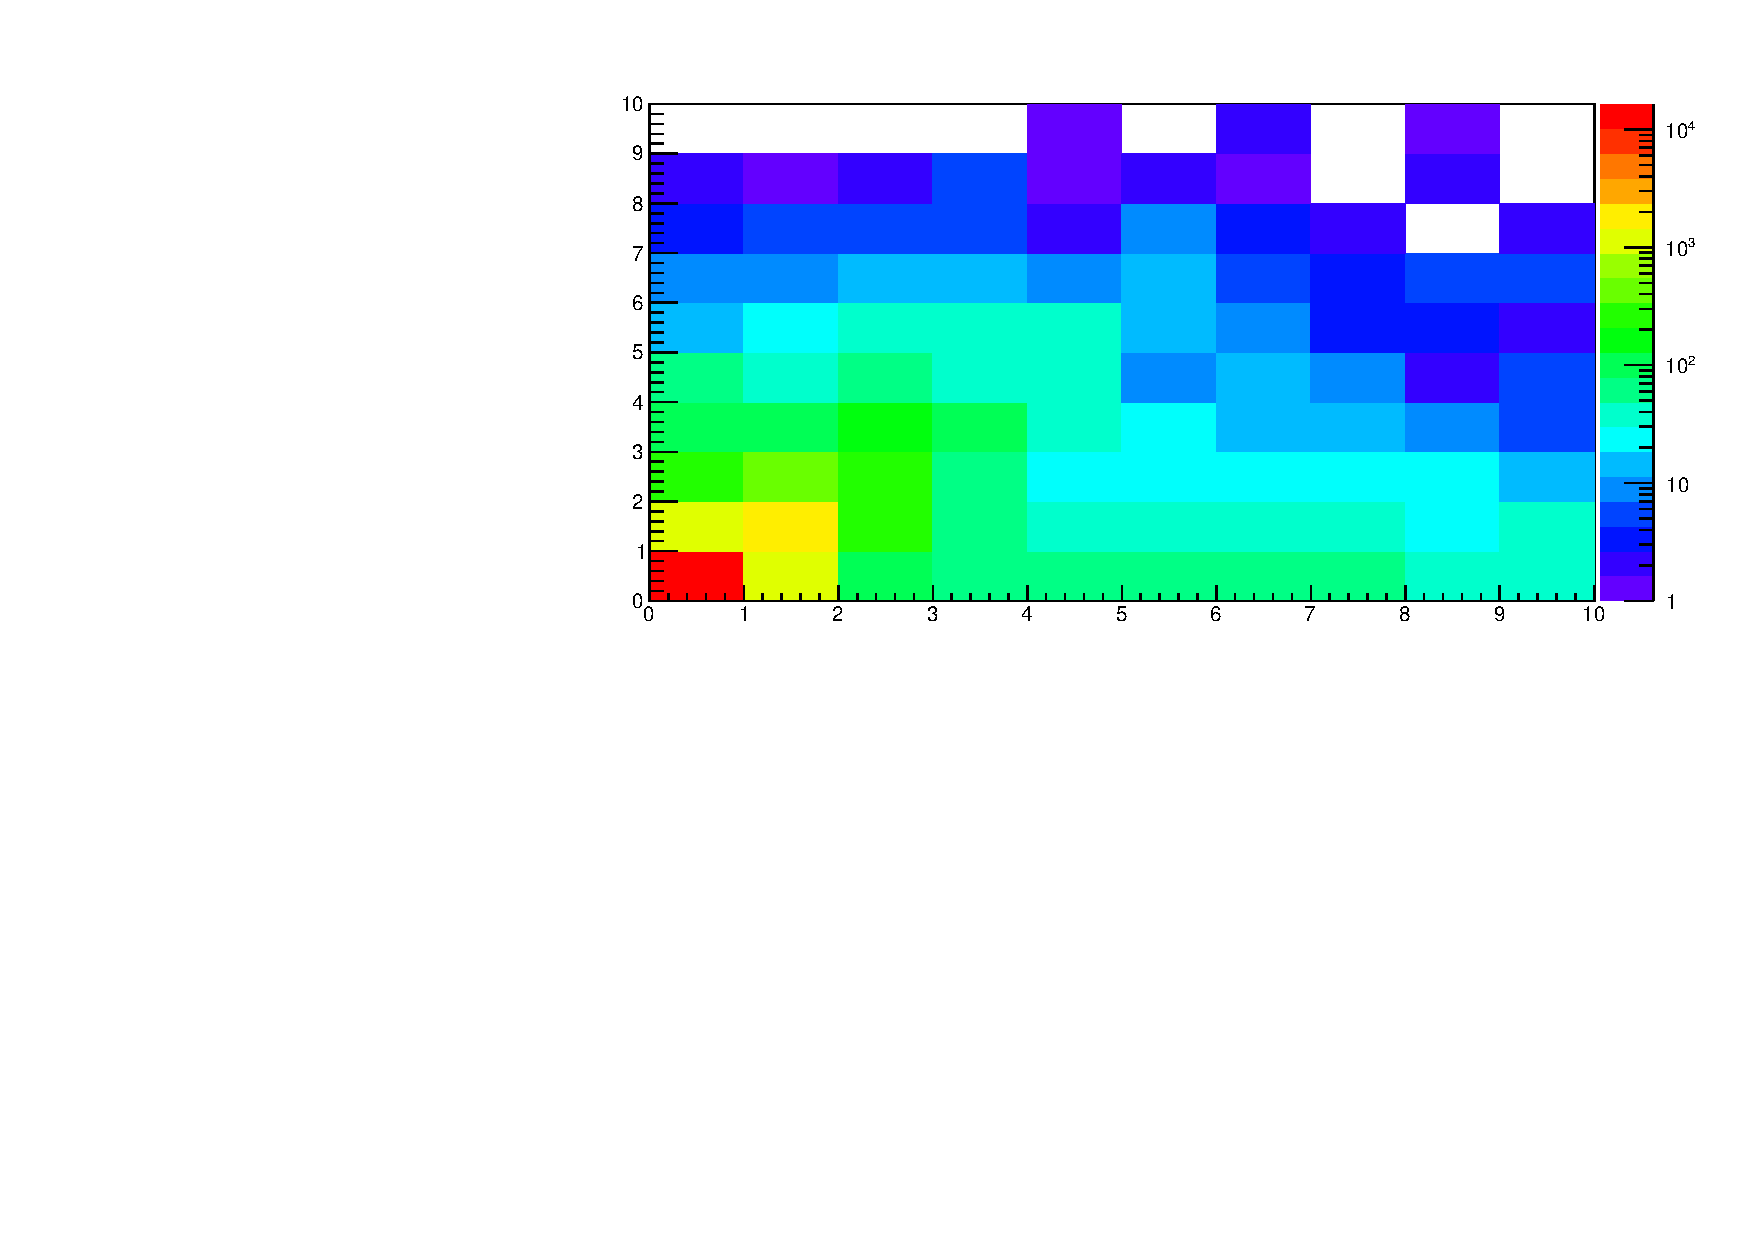
\includegraphics[scale=0.48,trim={5cm 0 0 0}]{Migration_E}
                \caption{10 Energy Bins, 1 Cos($\theta$) bin, 1 $\phi$ bin}
                \label{fig:mig_en}
    \end{subfigure}~~~~~~~~~~~~~~
    \begin{subfigure}{0.4\textwidth}
                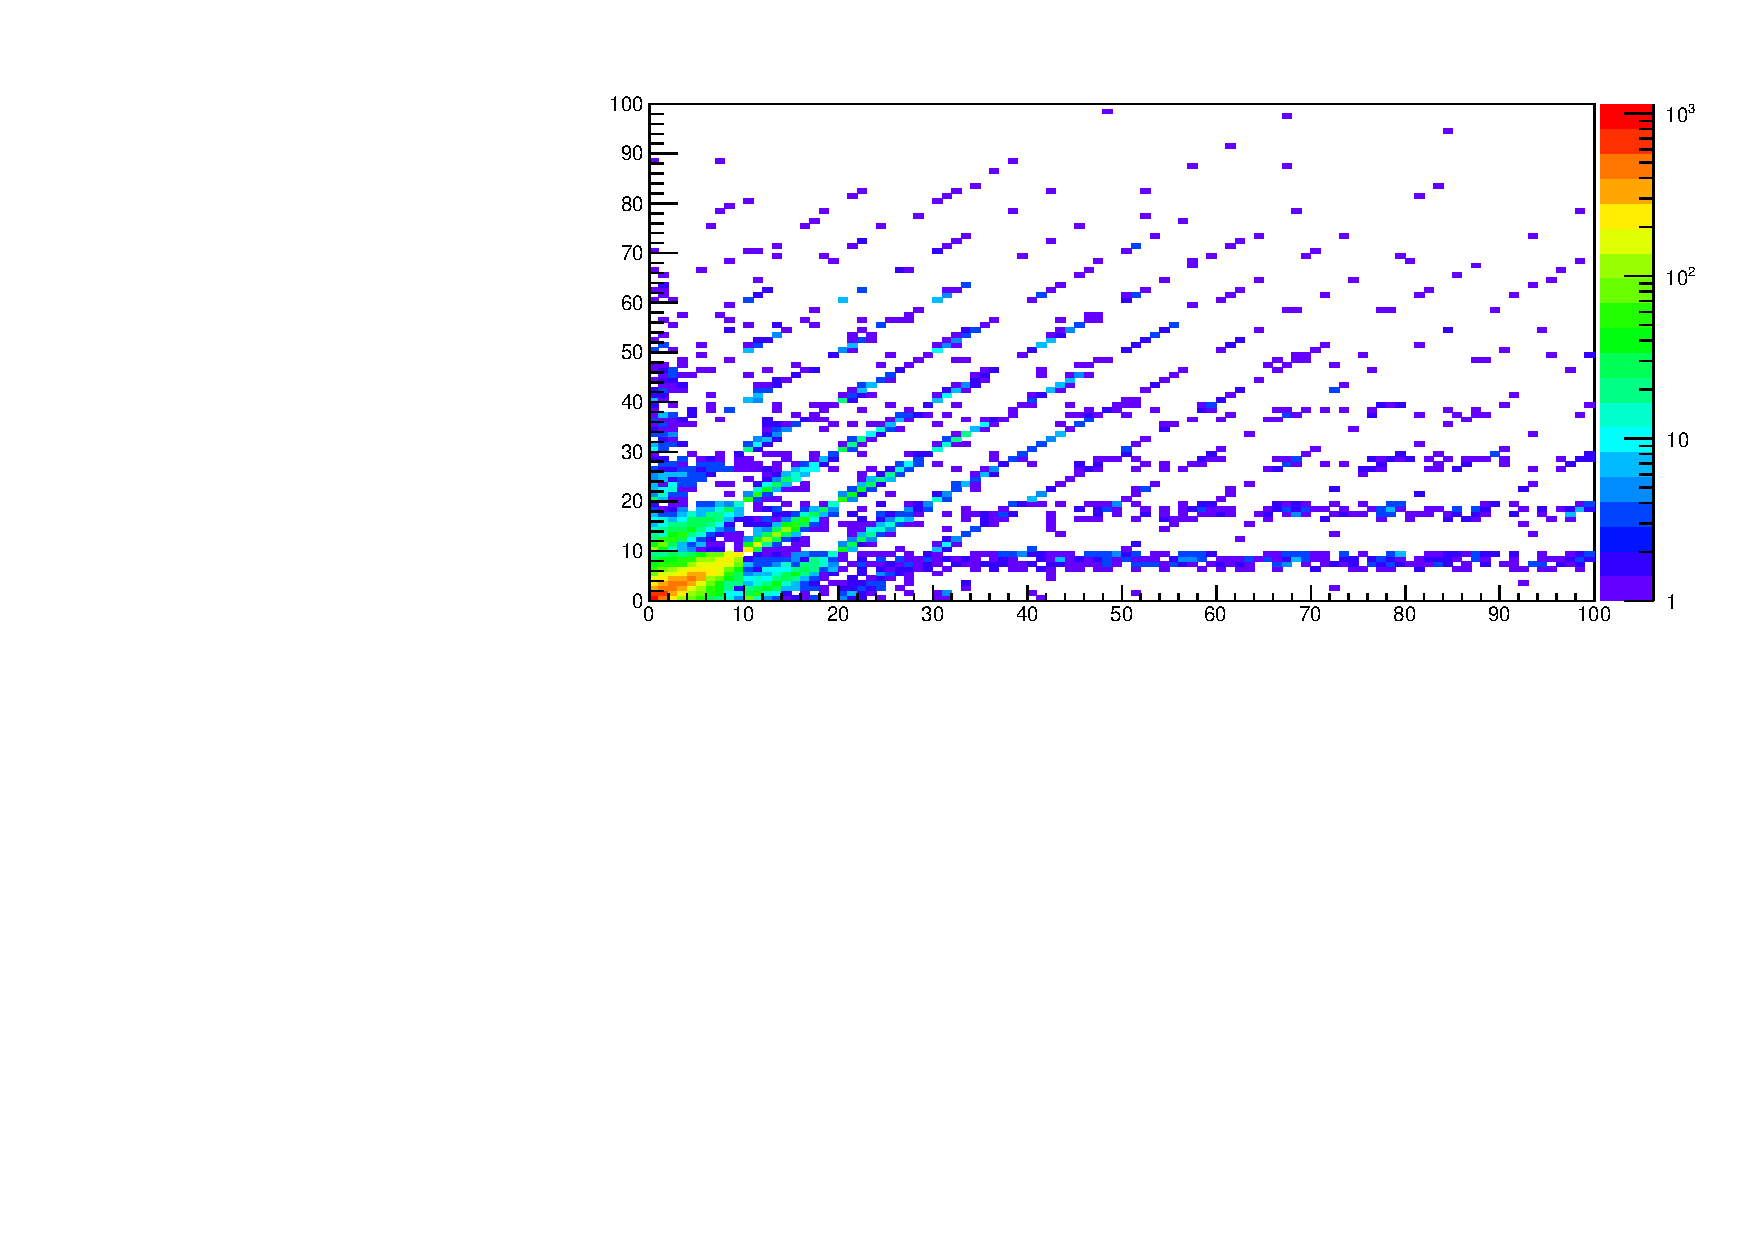
\includegraphics[scale=0.48,trim={2cm 0 0 0}]{Migration_E_Cos}
                \caption{10 Energy Bins, 10 Cos($\theta$) bins, 1 $\phi$ bin}
                \label{fig:mig_en_cos}
    \end{subfigure}\\
    \begin{subfigure}{0.4\textwidth}
                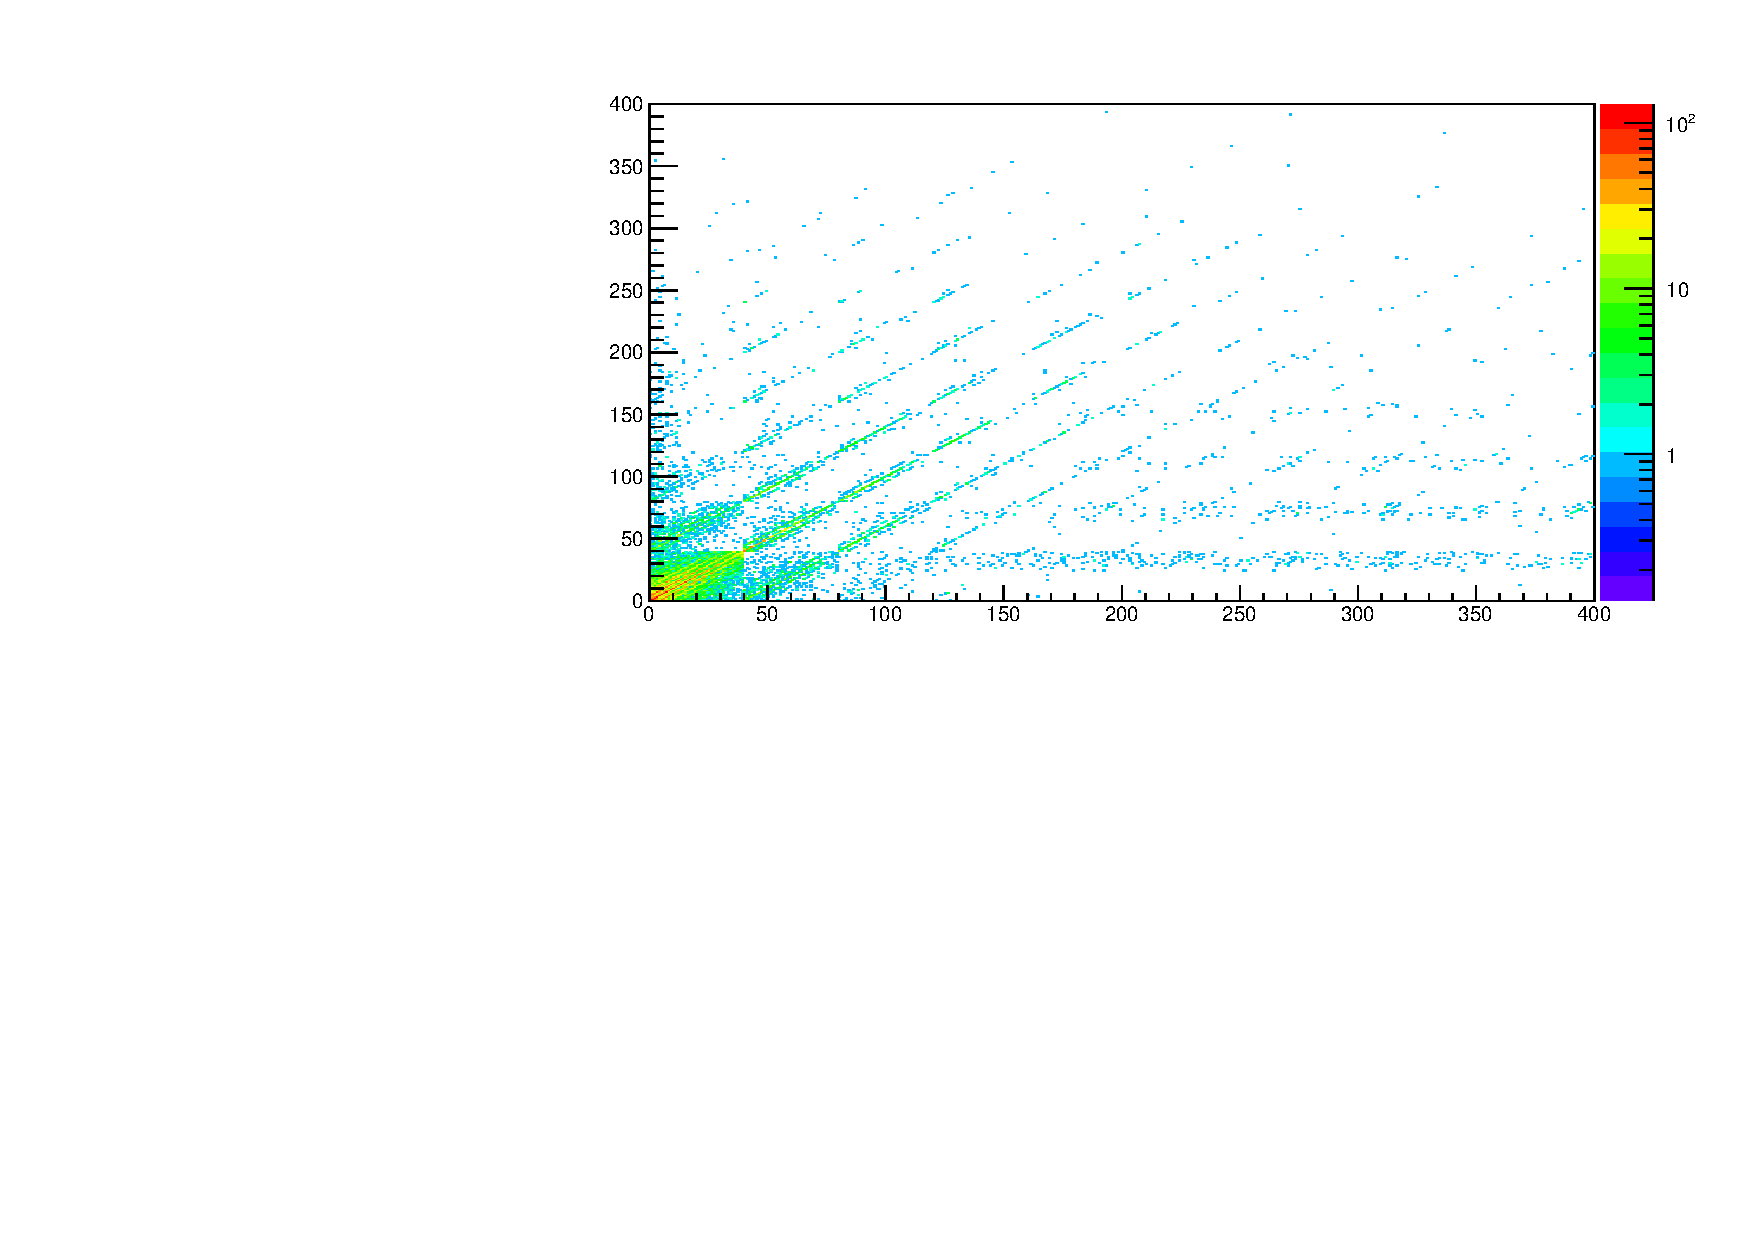
\includegraphics[scale=0.5,trim={5cm 0 0 0}]{Migration_E_Cos_Phi}
                \caption{10 Energy Bins, 10
                 Cos($\theta$) bin, 4 $\phi$ bins}
                \label{fig:mig_en_cos_phi}
    \end{subfigure}
	\caption{Different migration matricies, axis are simply bin numbers, in (\ref{fig:mig_en_cos}) every 10 bins are the cos($\theta$) bins for a given energy, in (\ref{fig:mig_en_cos_phi}) every 4 bins are $\phi$ bins for a given cos($\theta$) and a given energy.}
	\label{fig:migration_matricies}
\end{figure}
\begin{equation}
	U_{ij}=\frac{M_{ij}}{\sum\limits_k M_{kj}}.
\end{equation}
Now that we have the unfolding matrix we can start looking at the other components of equation (\ref{eq:DCS}).
%
%
\subsection{Number of Nuclei Targets}
The number of targets is hardcoded into the calculations. It was calculated assumed a cylinder of $R=600m$, $H=1200m$ and an average Antarctic ice density of $0.922Mg\,m^{-3}$.
This combined with the knowledge that the molar mass of $\text{H}_2\text{O}$ is $12.01528 g\,mol^{-1}$ we can calculate the number of $\text{H}_2\text{O}$ molecules using
\begin{equation}
	N = \frac{Vol \times \rho \times N_A}{n_{\text{H}_2\text{O}}} \approx 8.366\times 10^{37}
\end{equation}
where $\rho$ is the density of the ice, $N_A$ is Avagadro's number $n_{\text{H}_2\text{O}}$ is the number of moles of water.
\subsection{Other Variables} 
Finally we can just list off the other variables as they are all quite simple.
\begin{itemize}
	\item $d_j$ - this would be the post-detection data that we would be provided. As it is this is our fake data. Obviously if we just use the fake data we would just arrive back at our true data so we smear the fake data in the macro before we use it.
	\item $b_j$ - background data, this is any neutrinos that are non-atmospheric. In the simulation data there is not background and as such it has not been included in the code.
	\item $\Delta E$ - this is the energy bin width in GeV. The limits on energy for the histograms are hard coded to be [0,200] but the number of bins can be easily changed by the user.
	\item $t$ - time the simulation was run for. This was 3 years and has been hard coded into the calculation.
	\item $\Phi$ - This is the integrated flux density of neutrinos. One of the macros is written to explicitly calculate this and we will discuss this more in section (\ref{sub:calculating_integrated_flux}).
	\item $\epsilon_i$ - the detection efficiency is the probability of the detector detecting an event that occurred. It varies dependent on energy and angle, there is a mecro written to do this and we will discuss this more in sec(\ref{sub:calculating_detector_efficiency}).
	\item $Sr$ - the amount of solid angle included in this bin. Solid angle is measured with the integral of $\cos(\theta)$ and $\phi$ with integral limits of $[-1,1]$ and $[0,2\pi]$ respectfully, giving a maximum of $4\pi$ if all angular directions were considered at once. These are calculated by the initial bin number selection and do not need to be calculated by the user.
\end{itemize}

\section{Software Requirements} % (fold)
\label{sec:software_requirements}
There are a few pieces of software that you will need to have installed to be able to use the code this summary is about. The main one can only be installed on a linux machine so if you don't have one you will need to install a VirtualBox system. There is a lot of webpages mentioned in this section but they will all be included in the Useful Links section at the end of this summary.
%
\subsection{ROOT} % (fold)
\label{sub:root}
ROOT is a data analysis package created by CERN that allows for running of \emph{macros}, pieces of code that allow you to run long or complicated commands in ROOT without having to type them out each time. You can find instillation instructions on the ROOT main website as well as tutorials and help for how to use the package. However I would advise that you don't install ROOT just yet as you are going to have to do a special type of instillation for it when you go to install the next program.
%
\subsection{GENIE} % (fold)
\label{sub:genie}
GENIE is a monte carlo generator for neutrino interactions. It can be quite difficult to install from scratch but fortunately the creators of the program have written a script that \emph{should} install it all for you. If you go to the \emph{GENIEMC} github page there is a repo called \emph{lamp}; this script will install all the pre-requisites for GENIE and also GENIE itself, this includes ROOT. Helpful. You will need to make sure you are installing version 2.9.0 as this is the version the new flux driver you will need was written for. There is a chance that the install will fail if you don't have pre-requisites for the pre-requisites, I suggest reading the error message and finding out what is missing, or just google the error messages and hope to fix it. Good luck, you will need it.
%
\subsection{Honda Flux Driver} % (fold)
\label{sub:honda_flux_driver}
Whilst not currently implemented into the DCS code it was intended that you would be able to compare the weighted interactions with the Honda flux interactions generated by GENIE, that and if you are using this guide it's very likely that you would want to use Honda flux files to generate interactions with GENIE anyway. All that being said, GENIE can't read Honda flux files as it currently stands so you will need to download an edited version of the GENIE code to be able to run simulations with these flux files. Why did I have you install it via \emph{lamp} if I was just going to ask you to do it by hand anyway? Because the pre-requisite programs and paths are the hard parts to set up. So with this in mind, once again go to github but find the user \emph{rlh1994} and go to the \emph{GENIE\textunderscore 2\textunderscore 9\textunderscore 0} repo and the branch \emph{honda\textunderscore flux\textunderscore rv5318}. Once there you will have to download the entire folder as the file structure was changed from the publicly available 2.9.0 and this version, replace your current GENIE folder, make sure you're environment variables have been set correctly by typing \emph{source environment\textunderscore setup.sh} in your \emph{lamp} folder, then inside the GENIE folder type \emph{make}. It will take a while but it should completely rebuild GENIE with the new flux driver included.\\
\\
The other option to doing this is to set up the lamp installation such that it installs from this github repo and branch which may be easier depending on your experience with installing GENIE.\\
\\
Assuming there are no errors you have now correctly installed the new flux driver to allow GENIE to read Honda flux files. To run GENIE with these flux files, all the options for the \emph{gevgen\textunderscore atmo} command are the same except when specifying the flux file use \emph{ATMNC} instead of \emph{FLUKA/BGLRS} and if you wish to use simulate multiple neutrino types you must type the file name each time.
%
%
\section{File Package} % (fold)
\label{sec:code_package}
The macros that you will actually be running to calculate and plot the DCS is split into 4 programmes both for each of understanding and also to minimise run time. Each piece does small parts of the calculation and then the final piece combines all of the variables to give you the final DCS. Every effort has been made to require the least amount of editing from the user however, due to me not understanding how to give command line arguments easily in ROOT, there will be some editing that the user must do in each case to specify input file names and the number of each bin you would like. I have tried to make it so all the changes the user must make are close to the top of code and clearly commented. Whilst you don't need to understand how the code works the following will also explain some of the main methods the code uses and I made an attempt to comment the code so that users with some ROOT or C++ familiarity should be able to understand what is going on.
%
\subsection{Calculating the Migration Matrix} % (fold)
\label{sub:calculating_the_migration_matrix}
The first macro you will need to run is the one that will calculate the migration matrix as this will be used to get the true and fake data in the future using equations (\ref{eq:true}) and (\ref{eq:fake}). The code itself is called \emph{make\textunderscore complete\textunderscore histo.cpp} and will output a root file of the form \emph{icecube\textunderscore energy\textunderscore \#\textunderscore cos\textunderscore \#\textunderscore phi\textunderscore\#.root} where each $\#$ is the number of bins for energy, cos($\theta$) and $\phi$ respectively.\\
\\
This macro is the slowest running of all of them it runs with $\mathcal{O}(i^2j^2k^2)$ where i, j and k are the number of each set of bins which is obviously horrible if you want to add even just one more bin of any type. Fortunately if you don't want to change the number of bins or input file you will only need to run this macro once and the migration matrix is then saved to that output file, meaning you can quickly reconstruct the true or false data from the file without having to run this macro again.
\\
The two things the user has control over in this macro is the number of each type of bin and the input data file for the true and fake data. The first are easily identifiable variables declared immediately after the root variable initialising; they are \emph{nbins\textunderscore en, nbins\textunderscore cos\textunderscore theta} and \emph{nbins\textunderscore phi} which are the number of energy, cos($\theta$) and $\phi$ bins respectively. A few lines below this is when the input file is added and the user will need to change it so that it read their IceCube input file, the user will have to replace the current \emph{Level7\textunderscore genie\textunderscore ic.1460.0000XX\textunderscore LowE.root} with the name of their file.\\
\\
The code itself creates 2D sub-histograms from the true and fake data in the IceCube file using a series of cuts in the energy and the value of cos($\theta$) then places these into the main 2D histogram that represents the migration matrix where the content of each bin is the value of that matrix element. This histogram is then saved into the output file and will be used in most future calculations so please do not move this or any other output file to another folder. The matrix itself is currently formatted such that it cycles over the $\phi$ bins for each cos($\theta$) bin, and it cycles over the cos($\theta$) bins for each energy bin; so on the largest scale it looks like just the energy bins.
%
\subsection{Calculating Integrated Flux} % (fold)
\label{sub:calculating_integrated_flux}
The next thing that needs to be calculated is the integrated flux; this also only needs to be done once and is done with the file named \emph{honda\textunderscore integrate.cpp}. After this has been run it will create a file called \emph{integrated\textunderscore flux.dat} and this will be the same for all future calculations assuming you don't change the Honda flux file you use in GENIE. With that in mind the user will have to specify the flux file name that you wish to calculate the integrated flux for, you will need to replace the default \emph{kam-mu-nu-20-12-n3650.dat} with the name of your Honda flux file.\\
\\
The code itself does a very rough approach to working out the integrated flux; obviously it is impossible to get an accurate integral as you only have discrete data and as such we just calculate the combined area of the bins in the histogram. Bin edges for Honda files and the energy range of 3-195 are hardcoded into this program due to it only needed to be run once and for my purpose I didn't have to consider a different range as this is what IceCube simulations use. This macro is the one that will produce the most error just because of the data from the Honda flux not lining up with the IceCube simulation range.
%
\subsection{Calculating Detector Efficiency} % (fold)
\label{sub:calculating_detector_efficiency}
The efficiency of a detector is calculated simply by
\begin{equation}
	\epsilon_i = \frac{N^{after}_i}{N^{before}_i}
	\label{eq:effic}
\end{equation}
where $N^{after/before}_i$ is the number of events after/before cuts respectively. By cuts this includes anything such as the event not being detected, the computer deciding to not record the event etc. It is important to note here that whilst we calculated the total \emph{neutrino} flux, we are trying to calculate the DCS for the \emph{muons} and so the efficiency will be of the muon detection (as this is what IceCube actually detects anyway). The detector will have different efficiencies for different energies, zenith angles, and despite the fact it should be uniform over the azimuth angle we discovered there was some differences in efficiencies for these and as such we left the efficiency to be per energy, zenith, and azimuth (so technically it should be $\epsilon_{ijk}$ but we have wrapped the dimensions within each other). \\
\\
The macro itself, called \emph{ice\textunderscore genie\textunderscore loop.cpp}, relies on being passed 3 files: the migration matrix file, a file of neutrino events, and a file of anti-neutrino events. The latter two files must be of a 1:1 ratio, be generated with an $E^{-2}$ flux, with a target of water and with energies in the range 3-195 GeV. Two such files have been provided with the package as well as an extra macro that can generate files in the style of a FLUKA flux file if you wish to generate your own (although this isn't advised without a working knowledge of GENIEs flux driver code as it will involve editing that code, instructions for how to do this are provided in Appendix A, probably, it's probably A). \\
\\
As with most of these macros you will need to edit the three bin number values at the beginning of the code as well as changing the two root file names should you be providing your own. If you are providing your own and they do not total to 100k events you will need to change one more piece of the code; around line 86 at time of writing there is a line that says \\
\centerline{\emph{simulation\textunderscore histo-$>$Scale(300);}}\\
and you will need to change the 300 such that when multiplied by the total number of events in the files you have provided it equals to 30 million. If you used the provided files you will not need to change this line. The reason we have to scale this is because the IceCube simulation is actually 30 million simulated events to start with before all the cuts.\\
\\
The macro uses a very similar method to the one that was used to create the migration matrix to fill a histogram with the interaction file data and uses the migration matrix itself to get the true data (remember that the fake data is what we have \emph{reconstructed} the values for, the true data contains the values for the simulated events that were detected). Once it has these it simply uses equation (\ref{eq:effic}) to find the efficiency for that bin then writes these all out to a file of the form \emph{efficiency\textunderscore energy\textunderscore \#\textunderscore cos\textunderscore \#\textunderscore phi\textunderscore\#.dat} where the $\#$s represent what they did previously. Some examples of the efficiency as a function of energy, cos($\theta$) and $\phi$ are shown in figure \ref{fig:effieciency}.
\begin{figure}
	\centering
	\begin{subfigure}{0.4\textwidth}
                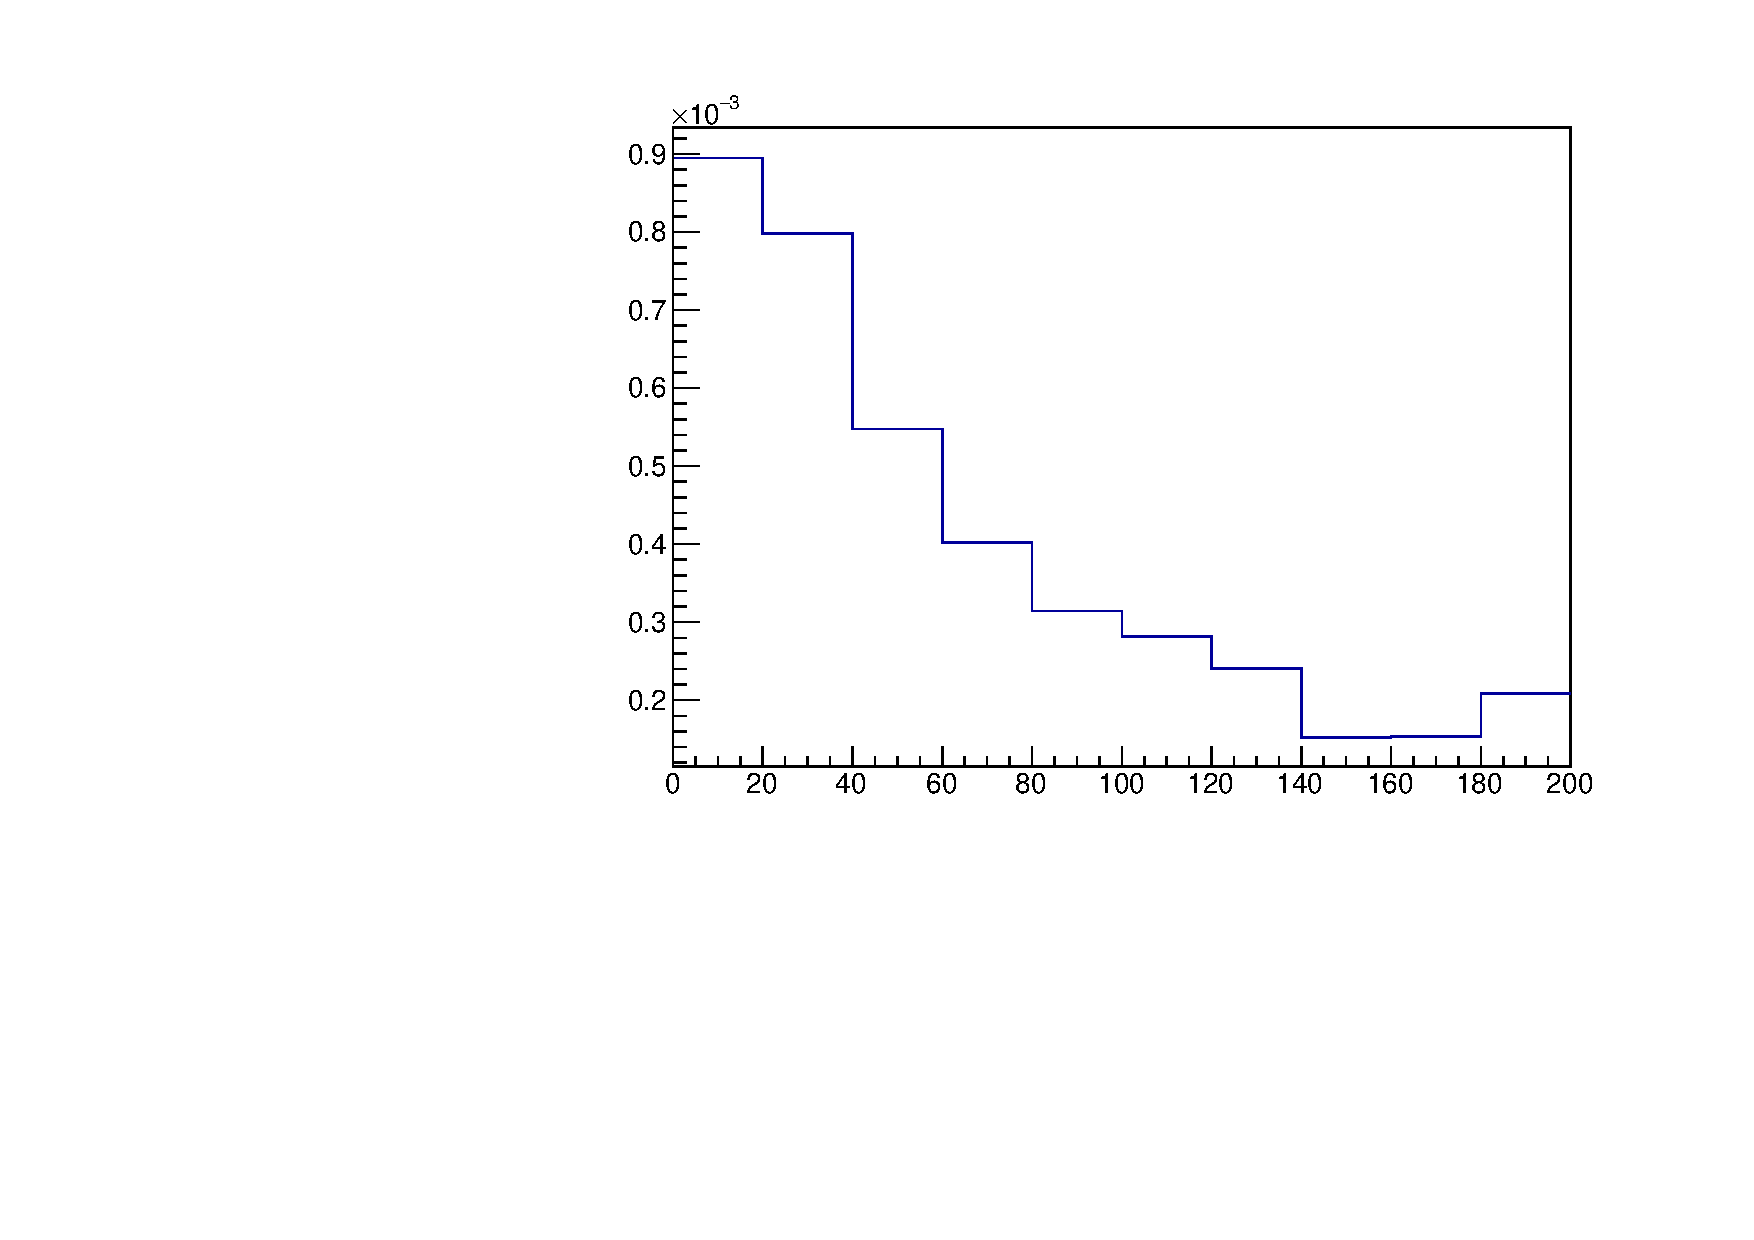
\includegraphics[scale=0.48,trim={5cm 0 0 0}]{Efficiency_en}
                \caption{Efficiency over 10 Energy Bins}
                \label{fig:eff_en}
    \end{subfigure}~~~~~~~~~~~~~~
    \begin{subfigure}{0.4\textwidth}
                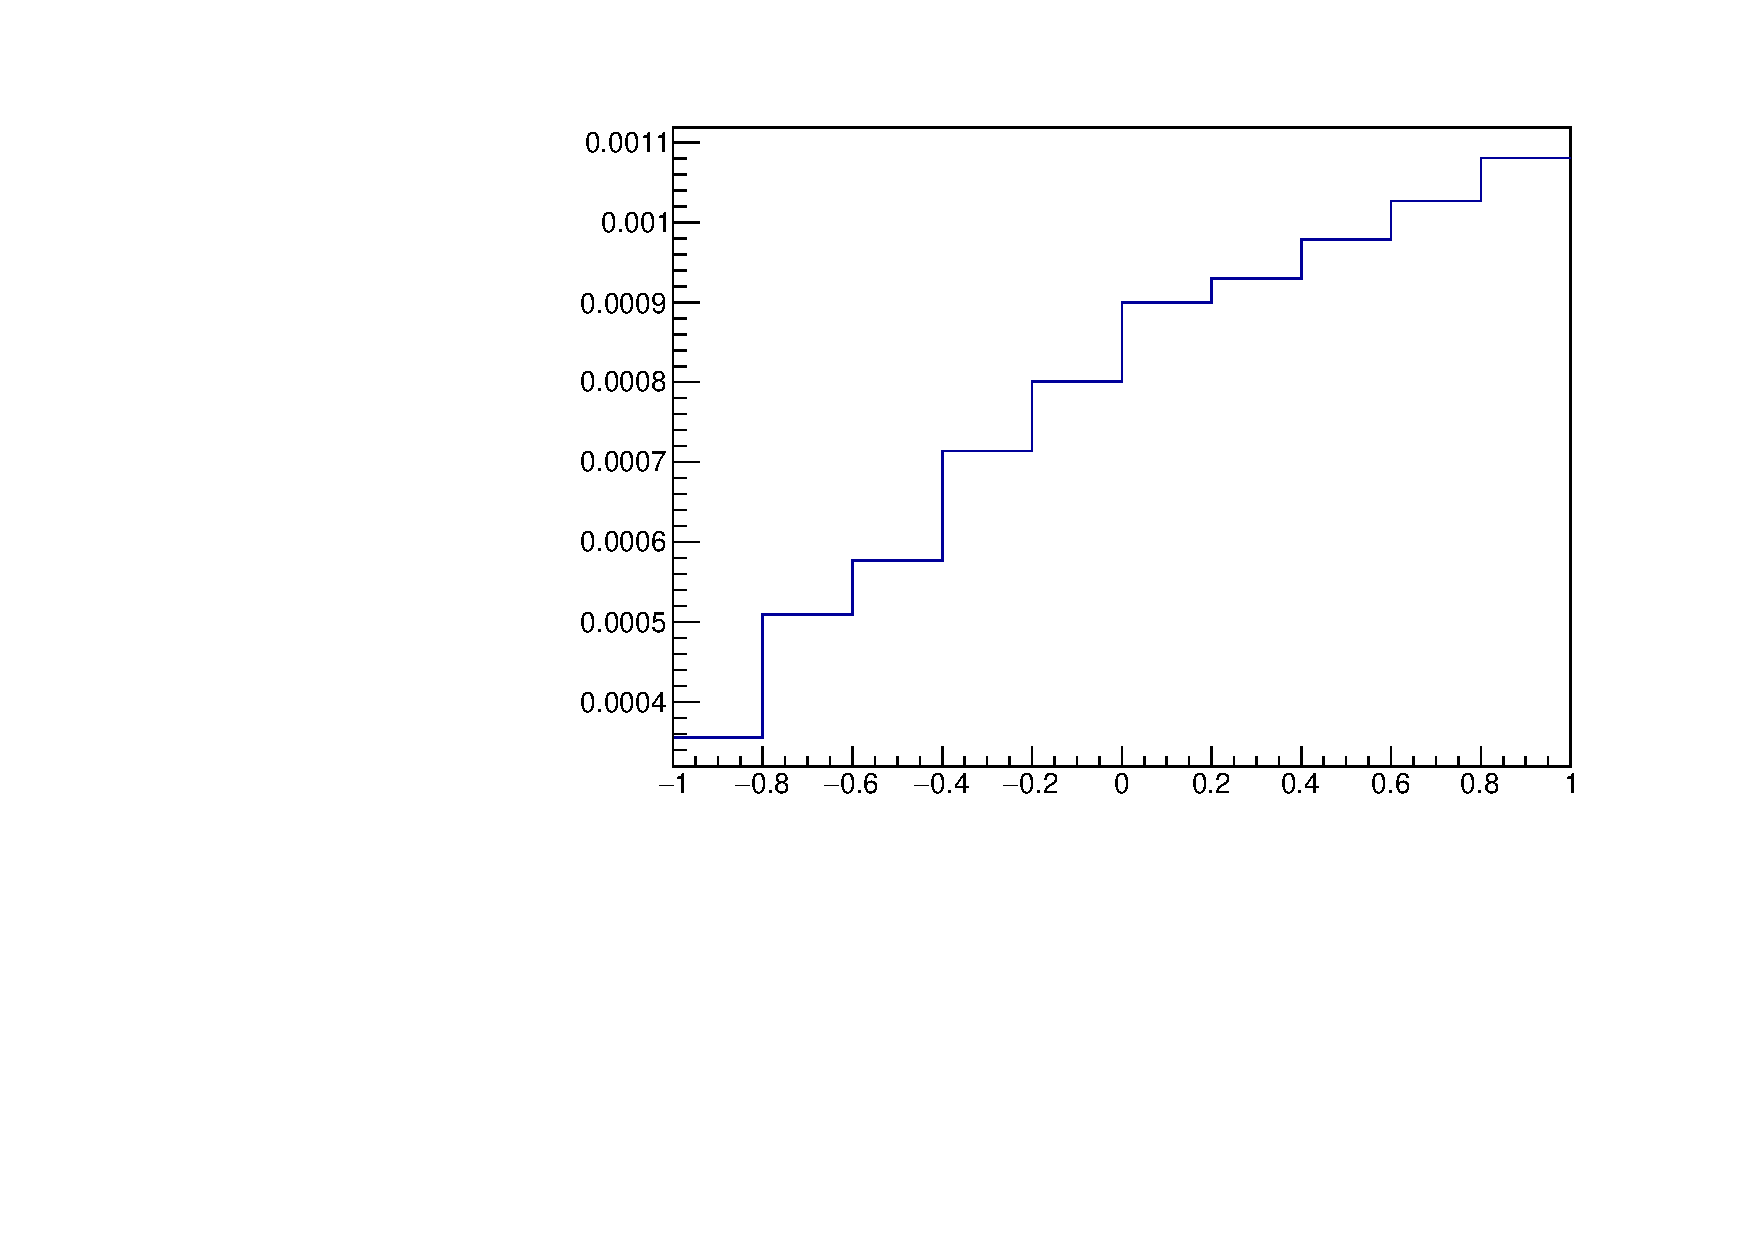
\includegraphics[scale=0.48,trim={2cm 0 0 0}]{Efficiency_cos}
                \caption{Efficiency over 10 Cos($\theta$) bins}
                \label{fig:eff_cos}
    \end{subfigure}\\
    \begin{subfigure}{0.4\textwidth}
                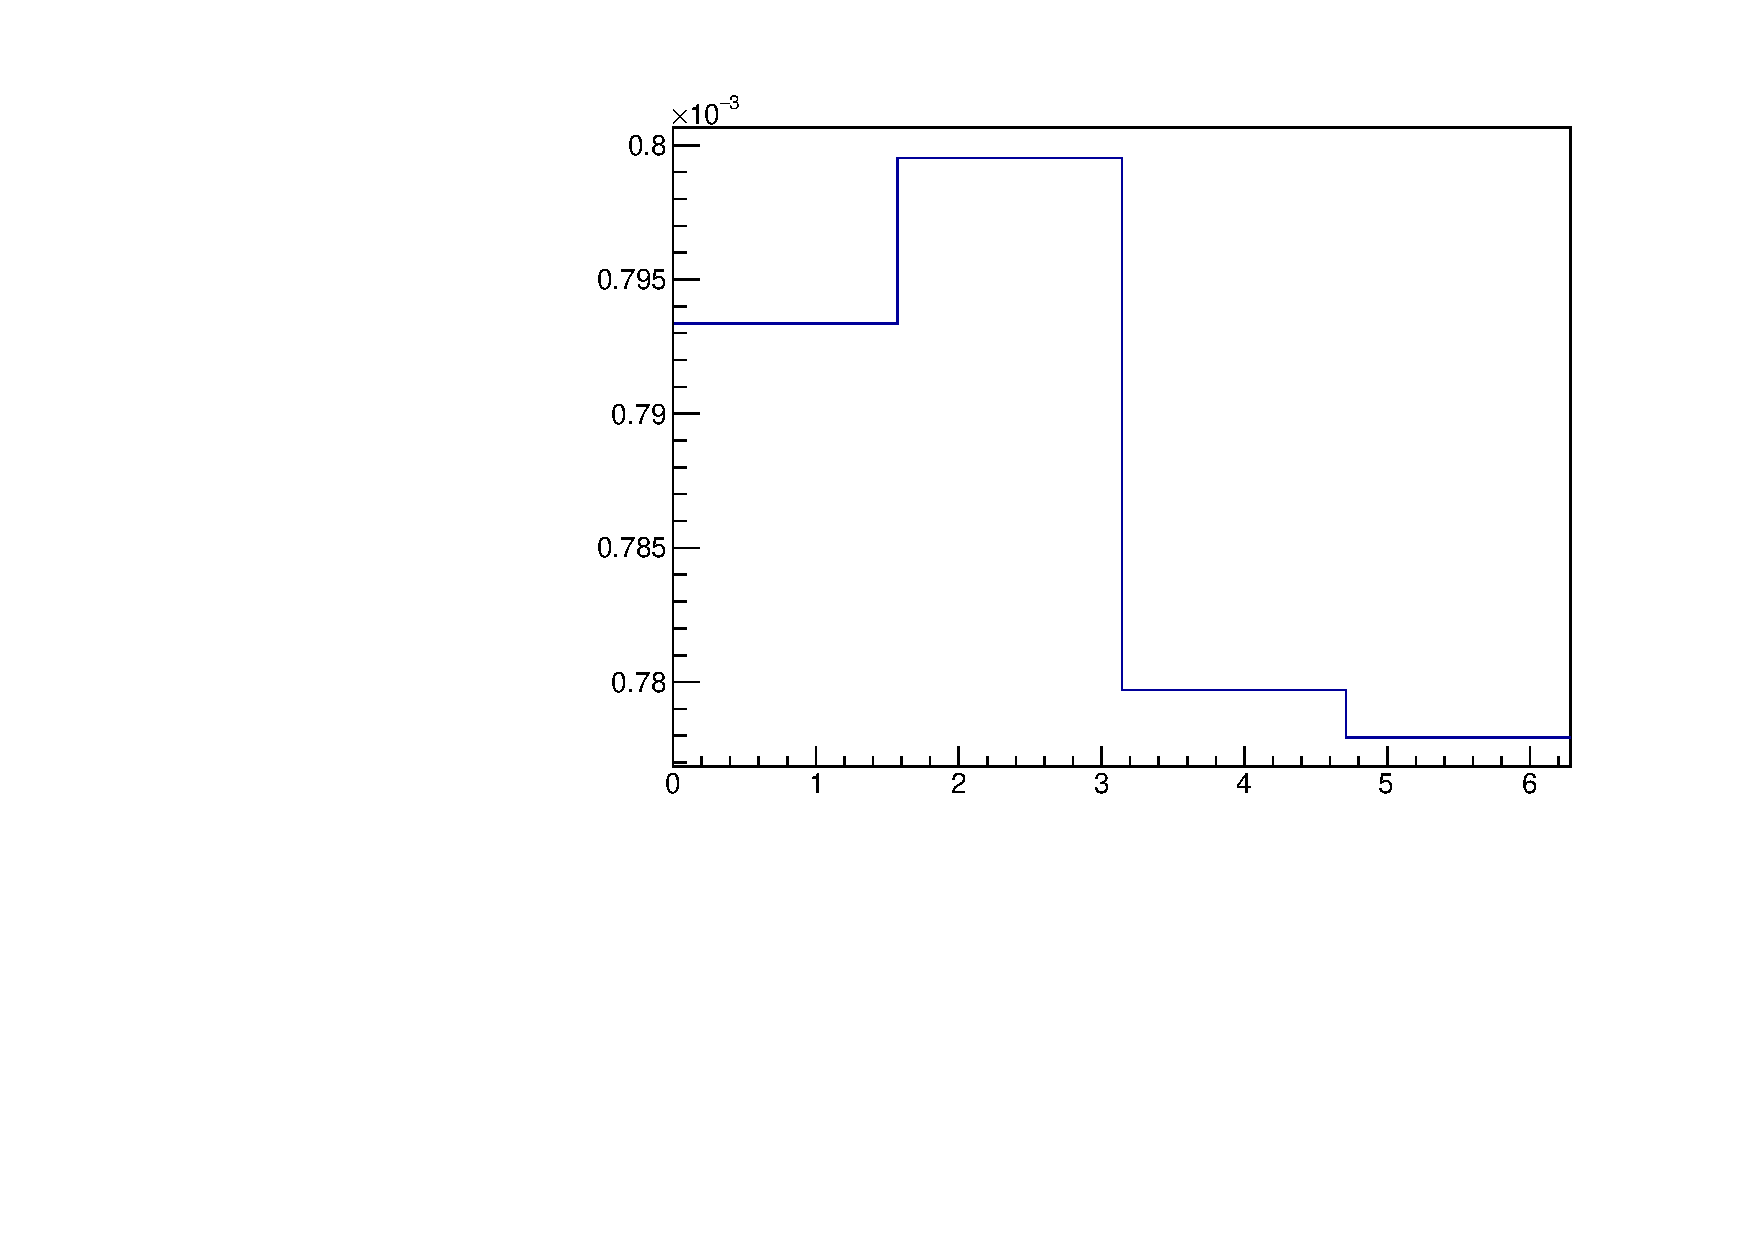
\includegraphics[scale=0.5,trim={4cm 0 0 0}]{Efficiency_phi}
                \caption{Efficiency over 4 $\phi$ bins}
                \label{fig:eff_phi}
    \end{subfigure}
	\caption{Efficiencies as functions of different variables. The later few energy efficiency bins are not reliable due to low statistics.}
	\label{fig:effieciency}
\end{figure}
%
\subsection{Calculating the DCS} % (fold)
\label{sub:calculating_the_dcs}
The final step to the calculation is just to combine all the parts into equation (\ref{eq:DCS}) and perform the sum, this is all done with the file named \emph{diff\textunderscore cross\textunderscore split.cpp}. Once run this macro will output two canvases, each with $m$ plots with $n$ histograms per plot, where $m$ is the number of cos($\theta$) bins, $n$ is the number of $\phi$ bins, all with the $x$-axis being energy in GeV. The first canvas titled \emph{MC Unfolded} is the one the user is likely to be interested in, it contains the histograms for the DCSs as functions of energy, cos($\theta$) and $\phi$, the second canvas titled \emph{MC Original} is in there to examine the phi dependence of the detector and was put in just for comparison, the user can feel free to ignore this canvas if it isn't required.\\
\\
Once again the user will be required to change the variables relating to the bin numbers at the top of the macro and they also have the option to change how the canvas is split for the plots as obviously this will vary depending on how many plots the user would want to have. To change the way the canvas is split the user would need to edit the lines that say\\
\centerline{\emph{c101-$>$Divide(5,2);}}\\
\centerline{\emph{c102-$>$Divide(5,2);}}\\
to contain whatever vertical and horizontal splitting numbers they want respectively (note that whilst there is no problem dividing the canvas into more plots than needed, the user will receive errors if there aren't enough divisions of the canvas). Currently there is no way for the user to have the plots printed to more than one canvas other than to change the code that plots the histograms which shouldn't be too difficult if the user has some familiarity with writing ROOT macros. 
%
\subsection{Other Included Files} % (fold)
\label{sub:other_included_code}
As mentioned previously there are a few other included files/macros to make it easier for the user to begin calculating DCSs. There are two ROOT files that contain GENIE simulated data to be able to run the efficiency calculation which are named \emph{genie\textunderscore energy\textunderscore cos\textunderscore 3\textunderscore 195\textunderscore numu\textunderscore 50k.root} and the same but with numu replaced with numubar. These files each contain 50000 events created using the set-up described in section (\ref{sub:calculating_detector_efficiency}) for $\nu_\mu$ and $\overline{\nu}_{\mu}$ respectively.\\
\\
The next file included is named \emph{flux\textunderscore create\textunderscore cos} because it creates a flux file in the FLUKA format using $\Phi(E,\cos(\theta),\phi) = E^{-2}$ i.e. only an energy dependence. This is the file that, when combined with the modifications to GENIE that can be made using Appendix A, will allow the user to calculate the efficiency for IceCube files with user defined energy limits. The user will need to change only one number in this file, the upper limit of the first for loop, to be equal to the base 10 logarithm of the highest energy they want (although I suggest going a few steps higher just to be safe). An example output file named \emph{e-2\textunderscore including\textunderscore cos.dat} has been included that goes up to 1000 GeV and can be used as an input for GENIE should you need to generate events of a higher energy. The IceCube simulations I had access to were generated with energies between 3 and 195 GeV, hence why only GENIE output files for that energy range were created and included.\\
%
%
\section{Next Steps} % (fold)
\label{sec:next_steps}
Whilst I believe that the work I have done is a good foundation for future work there are many gaps in the functionality of the macros as well as other problems I would have solved or options added were I to have more time. That being said what follows are just a few ideas of what could be done to expand/improve the work I started and there are certainly more options to consider than just those I will talk about here.
%
\subsection{Using More Files With TChain} % (fold)
\label{sub:using_more_files_with_tchain}
One task that was always pushed to the bottom of my to-do list was learning to properly use TChains; whilst they are used in the macros they are not used to the fullness of their ability. The first step would be to check all the places that the existing code uses TChains and make sure that is able to handle more than one file in that chain in all places. Once this is done more IceCube files could be included at once and this would increase the amount of data available at any one time which is always a good thing (this may change the scaling of the GENIE files in the efficiency calculation and that should be taken into account were you to include more IceCube files). The only other place work with TChains would be required is in the efficiency calculator where currently the neutrino and anti-neutrino simulations are in two separate TChains because of how I set up the combination of them later so this could be made more efficient by combining them into one TChain and modifying how the macro gets the values it needs from them.
%
\subsection{Weighted Events} % (fold)
\label{sub:weighted_events}
One thing that would be of great interest to look at would be the distribution considering a true neutrino flux. As it stands the IceCube data and the GENIE simulation are created by using an $E^{-2}$ flux and no other considerations are taken into account, but that needn't be the case. There is a variable saved in IceCube file that gives weighting to the events in agreement with Honda flux; to add this to the code is simple enough you simply need to multiply the entire cut string by the variable, namely \emph{AtmoWeightHonda.value} and this will give you the weighted distribution. The tricky part comes when trying to work out the efficiency because you need to correctly normalise the number of events before the cuts, i.e the GENIE simulation data.\\
\\
It was my understanding that the normalisation is linked to a constant that can be calculated by taking the events, dividing by the cross section and then finding the ratio between this distribution and that of the input Honda flux (or at least the average of the ratios for each bin) as 
\begin{equation}
	N \propto \Phi \otimes \sigma.
\end{equation} You then either divide or multiply the GENIE output by this and should in theory have normalised the number of genie events correctly. Unfortunately this gives a number that is horribly off what it should be. The problem is that I was not certain of what information the weighted IceCube data contained, I tried with just the cross section convoluted with the flux and multiplied by the time  of the simulation but this gave efficiencies of the order of $10^{-17}$ which was clearly incorrect. Anyone wanting to work on this would need to find the correct way to normalise the GENIE data by knowing what was included in the IceCube weighting, and then using this to calculate the new efficiency.
%
\subsection{Different Binning for True and Fake Data} % (fold)
\label{sub:different_binning_for_true_and_fake_data}
Something which I hadn't really considered until writing up this summary was that a user might want to have different binning for true and fake data and as such the code is written throughout to work with a square migration matrix. A next step in the work could be to make it so that the migration matrix could be a non-square matrix and this would involve modifying pretty much every for loop in all the macros that use the number of bins as a limit in one way or another. This would be useful for the reasons I explained in section \ref{sub:unfolding_matrix}.
%
\subsection{Optimisation of the Code} % (fold)
\label{sub:optimisation_of_the_code}
As it stands some of the code is horribly inefficient; a lot of it was just made to work before carrying onto the next step and as such there are probably many places where the code could be optimised to run faster/more efficiently.\\
\\
The bottleneck of any run is in generating the migration matrix; this takes by far the longest of any of the macros and runs at $\mathcal{O}(i^2j^2k^2)$ where i, j and k are the number of each set of bins. This is obviously not going to be useful if you want to take a large number of bins, as it stands even small numbers of bins can take a long time to run. This should be the main starting point for any code optimisation as even if other parts of the code were improved this would still be the part a user was waiting on.\\
\\
The method by which the migration matrix is made involves, as mentioned previously, creating small histograms, getting the bin content, then setting this content into the larger histogram; this method is applied throughout all the macros and if it were improved upon in one could almost certainly be improved upon in the others as this is the part of the macros that takes the longest to run in each case.
%
%
\section{Conclusion} % (fold)
\label{sec:conclusion}
The work I have done over the summer has created a very good foundation to calculate DCSs from IceCube files. There are ways in which the macros would be improved, both in efficiency and customisation, but there is enough there for now that it can at least do the calculations. I think these macros have a lot of potential in use for a variety of applications and could be very useful with just a few more additions to their capabilities, namely adding the ability to do weighted calculations and reducing the time it takes to run the migration matrix generator.
%
\section{Useful Links} % (fold)
\label{sec:useful_links}
ROOT: \url{https://root.cern.ch}\\
GENIE main site: \url{http://genie-mc.org}\\
Lamp github page: \url{https://github.com/GENIEMC/lamp}\\
Honda Flux Driver github page: \url{https://github.com/rlh1994/GENIE_2_9_0/tree/honda_flux_rv5318}\\
VirtualBox download: \url{https://www.virtualbox.org}\\
IceCube website: \url{http://icecube.wisc.edu}\\
Honda flux files: \url{http://www.icrr.u-tokyo.ac.jp/~mhonda/}\\
\newpage
\appendix
\section{Modifying GENIE to use larger FLUKA files} % (fold)
\label{sec:appendix_a_modifying_genie_to_use_larger_fluka_files}
As talked about in section \ref{sub:other_included_code} we can generate a FLUKA flux file with a custom flux function and an arbitrary energy range. The problem in trying to use these is that GENIE expects to receive a FLUKA file with 61 energy values per cos($\theta$) range and as such will not work if we just try to give it a file with a higher energy range. Fortunately the code is quite easy to change and only requires one modification as long as you leave the minimum energy and the energy steps the same, only changing the maximum energy value in the file. To pick the maximum energy you must take the base 10 logarithm of the energy, add one more step size to it, then set this value as your upper limit in the first for loop in the file. \\
\\
If you are currently in the top level of your GENIE directory (not the lamp folder but the actual GENIE\textunderscore 2\textunderscore 9\textunderscore 0 folder) then the file you are going to edit is\\
\centerline{ \emph{src/FluxDrivers/GFlukaAtmo3DFlux.h}}\\
so open that up in your editor of choice and then find line 50 which should be\\
\centerline {\emph{const unsigned int kGFlk3DLogNumEvBins       = 61;}}\\
which just means that there is a total of 61 bin energies given that are logarithmically spaced. Replace the number 61 with the number of steps your first for loop in \emph{flux\textunderscore create\textunderscore cos} remembering that a for loop uses [min, max), i.e. it doesn't use the maximum value. As it currently stands the for loop uses steps of 0.05 so to calculate the number of steps you take you can just use 
\begin{equation}
    n_{Steps} = (i_{max} - i_{min})\times 20.
    \label{eq:steps}
\end{equation}
This equation will work if you have changed the minimum energy value which we will talk about in a second, but will not work if you have changed the step size.\\
\\
The following steps have not been tested and can't be guaranteed to work so proceed at your own risk.\\
\\
If you wish to change the minimum energy value to be lower than 100MeV, you will have to follow the same steps above to find the minimum value required in the for loop, except you will just use the base 10 log value as the minimum in included in the loop, compared to the maximum which is not. In the same file as above you will also have to change line 52,\\
\centerline {\emph{const unsigned int kGFlk3DEvMin       = 0.100;}}\\
and replace 0.100 with your minimum energy value in GeV then recalculate the number of bins you have and make sure that number has been correctly changed.\\
\\
Finally if you wish to change the step size for more or less detailed flux data then you will need to change the step size in the for loop, remembering that these are log energy steps. Once you have changed this you will need to change the number of bins because equation (\ref{eq:steps}) becomes
\begin{equation}
    n_{Steps} = \frac{i_{max} - i_{min}}{step\textunderscore size}.
\end{equation}
You will also need to change line 51 which is usually\\
\centerline{\emph{const unsigned int kGFlk3DLogNumEvBinsPerDecade       = 20;}}\\
and replace the 20 with 1 divided by the step size.\\
\\
Once you have made any changes that you require you will need to make GENIE again as before, although this time it will be much quicker as it only has to rebuild the parts you have changed. GENIE should now accept your modified FLUKA file, I recommend you run a short test to make sure that everything is working correctly and you get a correct looking histogram for the output data. Finally, make sure if you want to use a normal FLUKA file after this you change the numbers back and make GENIE once more.
% section appendix_a_modifying_genie_to_use_larger_fluka_files (end)
%
%
%
%
%\nocite{*}
%\bibliographystyle{ieeetr}
%\bibliography{solitonbib} 
\end{document}